

Toutefois, des descriptions de configurations spatiales parfaitement
inéligibles pour le locuteur humain, comme \enquote{La boulangerie à
  côté de chez moi fait les meilleurs croissants de Paris}, peuvent
être extrêmement difficiles à interpréter informatiquement.

La transformation d'une description de position en une zone définie
par des coordonéess

%-> geo-information
\emph{Geographic Information Retrieval} \autocite{Jones2008}


%-> transition secours en montagne "le problème devient grave"

La difficulté de cette opération peut devenir critique lorsqu'elle
impacte les secours à la personne \autocite{DosSantosFerreria2019} 

% -> transition choucas
Les unités de secours en montagne \acp{usem} sont également soumises
à ces problèmes de localisation

Le projet de recherche Choucas, auquel cette thèse se rattache

% Présentaiont thèse
Un tel objectif soulève nécessairement de nombreuses questions, comme
l'importance que prend le XX

% inteprétation sémantique

% spatialisaiton

% fusion
Il est également nécessaire de se demander comment regrouper toutes
les spatialisations d'une alerte pour construire la zone correspondant
à l'ensemble des descriptions données par le réquérant et don à la
position de la victime.

% prise en compte imprécision

% incertitude



% Pas de Tal
Notre propos n'est cependant pas de travailler sur le \emph{traitement
  automatisé des langues} (TAL), 

%\begin{figure}
%   \centering
%   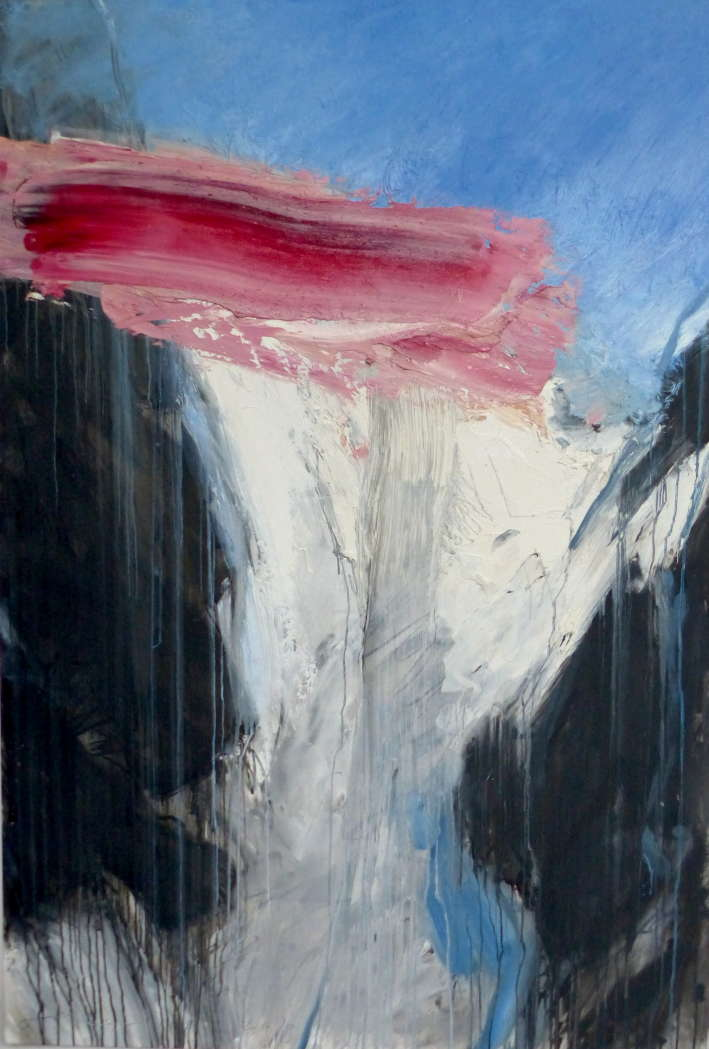
\includegraphics{./figures/Le_couloir_Rochette.jpg}
%   \caption{\emph{Le couloir,} Jean-Marc \bsc{Rochette,} 2010.}
%   \label{fig:couloir_rochette}
% \end{figure}

\addsec{Organisation du manuscrit}

Notre mémoire de thèse est organisé en trois parties, totalisant neufs
chapitres. Dans la \autoref{part:01} nous présenterons le cadre
général dans lequel notre travail s'inscrit. Le premier chapitre sera
dédié a la présentation du contexte applicatif et organisationnel de
cette thèse. Nous détaillerons le rôle et le fonctionnement des
secours en montagne, les problèmes soulevés par la localisation des
victimes et la manière dont le projet CHOUCAS souhaite y répondre. Le
second chapitre est destiné à présenter le contexte de scientifique et
la problématisation de notre thèse. Enfin, dans le troisième chapitre
nous dresserons un état de l'art sur les questions principales de ce
travail.

La \autoref{part:02} est destinée à présenter notre méthode de
transformation des positions exprimées dans un référentiel indirect en
des zones de localisation. Elle est constituée de cinq chapitres. Le
premier chapitre de cette partie présente l’organisation générale de
notre méthode. Les chapitres suivants approfondissent des points
spécifiques de cette méthode. Dans le \autoref{chap:05} nous
détaillerons le fonctionnement de la première phase de la méthode,
\emph{la décomposition.} Le \autoref{chap:06} sera quant à lui
consacré a la définition d'un modèle permettant la représentation
d'objets géographiques imprécis, tels que ceux produits par notre
méthode. Dans le \autoref{chap:07} nous présenterons la seconde phase
de notre méthode, \emph{la spatialisation.} Le dernier chapitre de
cette seconde partie sera consacré à la présentation de la dernière
phase de notre méthode, la \emph{fusion.}

Enfin, la \autoref{part:03} de ce manuscrit présente l’application de
la méthode définie a plusieurs alertes réelles. Cette partie ne
contient qu'un seul chapitre, le neuvième, où notre méthode est
appliquée à la modélisation de trois alertes réelles.


%%% Local Variables:
%%% mode: latex
%%% TeX-master: "../../main"
%%% End:
